
\chapter{引言}
\label{chap:Introduction}

\section{课题研究的背景和意义}
\label{section:background}
%加速器是什么?
粒子加速器是一种可以使带电粒子在高真空场中受磁场力控制、电场力加速而达到高能量的装置。
作为为基础科学研究提供条件的工具,粒子加速器在理解各类原子核结构、原子核内部的相互作用,以及研究天体物理、宇宙学、生命科学、材料科学、核医学等方面都有着重要的意义。
粒子加速器最开始的用途是高能物理研究,目标是研究粒子的微观结构和发现新的物理现象。
高能物理和粒子物理研究中所用的粒子对撞机就是一种加速器,
比如CERN的LHC(Large Hadron Collider)、
日本KEK的SuperKEKB、
美国BNL的RHIC(Relativistic Heavy Ion Collider)、
中国的北京正负电子对撞机(Beijing Electron–Positron Collider II,BEPCII)等等。

%加速器的一些应用和分类
除了在高能物理方面,加速器在其他方面也有着许多应用。
粒子加速器可以用作同步辐射光源,比如美国ALS(Advanced Light Source)、上海同步辐射光源、
以及北京在建的新光源等。此类的光源装置在物理、材料、化学、生物、医学等方面发挥着越来越重要的作用;
加速器还在医疗方面有很多应用,比如质子加速器是目前最有效的治疗癌症的装置;
除此之外,加速器还在新能源研究中起到重要作用,比如加速器驱动的次临界洁净核能
系统(Accelerator Driven Sub-critical System,ADS)是目前产生
核能、增殖核材料和嬗变核废物的解决方案之一。

%加速器的分类
粒子加速器的种类很多,它们的特点各有不同,可以按不同的原则加以分类。
按照粒子运动的轨道形状分,加速器可以分为环形加速器和直线加速器。
按照加速粒子的种类划分,可以分为电子加速器,离子加速器。
本论文的主要研究范围是强流离子加速器。

%我们要研究的是“强流”加速器
因为加速器中的大部分实验事例与加速器束流流强正相关,所以强流加速器成为了未来的加速器科学重要的发展方向之一。
强流加速器在核物理、生命科学、材料科学等基础科学研究,以及核医学、放射医学等应用研究方面有着越来越重要的作用。
在最近二十年来,得益于高能物理、核物理、散裂中子源、加速器驱动的次临界核能系统以及其它应用领域的强烈需求,强流粒子加速器也得到了较大的发展\cite{wei2003synchrotrons,chou2002synchrotron}。而随着加速器朝着高流强的方向发展,我们也面临着新的问题和挑战。
%所有的这些需求,都在推动着加速器往更高流强发展。

%强流束流动力学:空间电荷,集体效应
强流束流动力学主要研究的是加速器中的大量带电粒子在自生库伦场和外界电磁场中的演化问题。
强流离子加速器的一个特点是粒子束流受空间电荷效应的影响很大,导致束流的集体不稳定性较为突出,从而导致束流的整体损失或束流品质变坏。
空间电荷效应是指束团内部粒子之间的库仑作用,其作用的来源为带电粒子本身。
束团中的粒子带相同的电荷,相互排斥,会受到其他带电粒子的斥力,导致带电束团的自然发散和粒子的相位改变。
而集体不稳定性的来源有两个,一个是空间电荷效应,一个是加速器的外部环境,
比如束团与弯转磁铁,聚焦磁铁,加速腔等的相互作用。
空间电荷效应和束流的集体不稳定性都可能导致束流的品质变差或者产生束损。

%为什么要研究空间电荷,引入束损
在加速器中研究空间电荷效应的目的主要是提升束流品质,控制束损。空间电荷效应和束流流强,束流能量,以及束团的大小有关。
在现有聚焦强度下,流强越强,空间电荷效应带来的问题越严重,
特别实在束流能量低流强大的时候,空间电荷效应非常明显。
如果不加以控制,束流损失会很大。
随着束流流强和能量的提高,即使很小的束流损失也会使机器维护无法有效进行、实验条件无法得到保障,
所以束流损失率的控制也必须更加严格。
国际上流行采用平均损失率为1 W/m的手动维护标准,这个标准最早是针对1 GeV量级的质子束流能量,但对较低的束流能量也基本上适合。
譬如,对于能量为1 GeV、平均流强为1 mA的质子束,允许的束流损失率为1 nA/m或$10^{-4}~\%$/m。
这个要求非常严格,需要从物理设计和技术措施两方面上保证实现。

%强流束流动力学的难点:空间电荷效应
强流束流动力学研究的主要问题,也是难点问题,是如何自洽的表述束流自身产生的非线性空间电荷效应。
空间电荷效应导致的束流和粒子的共振和不稳定性、不同自由度之间的发射度交换、束晕粒子的产生、束流丢失等问题成为了强流束流物理中关注的焦点。
如何定性,定量理解强流束流动力学中的由于非线性空间电荷效应导致的束流集体不稳定性、束晕粒子形成机制也成为了近年来加速器物理研究中的重要课题。
%如何解决:物理图像上,数值上
这些问题背后的物理机制可以从物理模型和数值模拟两方面进行了研究。
从物理模型方面,非自洽的空间电荷模型可以被用来对其进行分析,以得到粗略的物理图像。
然而,空间电荷效应是一个多体的耦合问题,无法得到解析解。
为了更加精确地探寻其背后的物理机制,数值模拟是必不可少的。
而为了获得更为精确地物理图像,粒子模拟程序的运行效率必须进行提高。

为了进一步提升模拟程序的运行效率,我们考虑对其进行并行化处理,并比较了不同的并行架构。
GPU英文全称为Graphic Processing Unit,中文为“图形处理器”。
GPU一开始是由于在现代的计算机中图形的处理变得越来越重要,需要一个专门的图形核心处理器,
使显卡减少对CPU的依赖,并进行部分原本CPU的工作;
CPU是英文全称为Central Processing Unit,中文为“中央处理器”,一般由逻辑运算单元、控制单元和存储单元组成。
近年来,GPU高速发展,极大的提高了计算机图形处理的速度和质量,不但促进了图像处理、虚拟现实、计算机仿真等相关应用领域的快速发展,同时也为人们利用GPU进行图形处理以外的通用计算提供了良好的运行平台。

相对于CPU,GPU在并行处理和计算密集型问题方面具有很大优势。目前,GPU已成为普通计算机强大、高效的计算资源。如图\ref{fig:GPU}所示,一个CPU一般只拥有少数几个核,而一个GPU会有几百甚至几千个核。从系统架构上看,GPU针对向量计算进行了高度并行的数据流优化处理,这种多核架构特别适合进行数据并行。这种以数据流作为处理单元的机制,在对数据流的处理上可以取得很高的速度。
GPU 加速计算是指同时利用GPU 和 CPU,加快应用程序的运行速度\cite{gpu2008}。GPU厂商为科学计算设计了自己的API,其中CUDA(Compute Unified Device Architecture)就是NVIDIA设计的并行计算平台和编程规范\cite{nvidia2010programming}。利用CUDA,我们能够有效的利用GPU,使程序的运行效率大大提高。

根据使用CUDA的测试结果显示,利用GPU实现FFT(Fast Fourier Transformation)、BLAS(Basic Linear Algebra Subprograms)、排序及线性方程组求解等科学计算,与单纯依靠CPU实现的算法相比,平均性能提高了近20倍。
\begin{figure}[!htb]
    \centering
    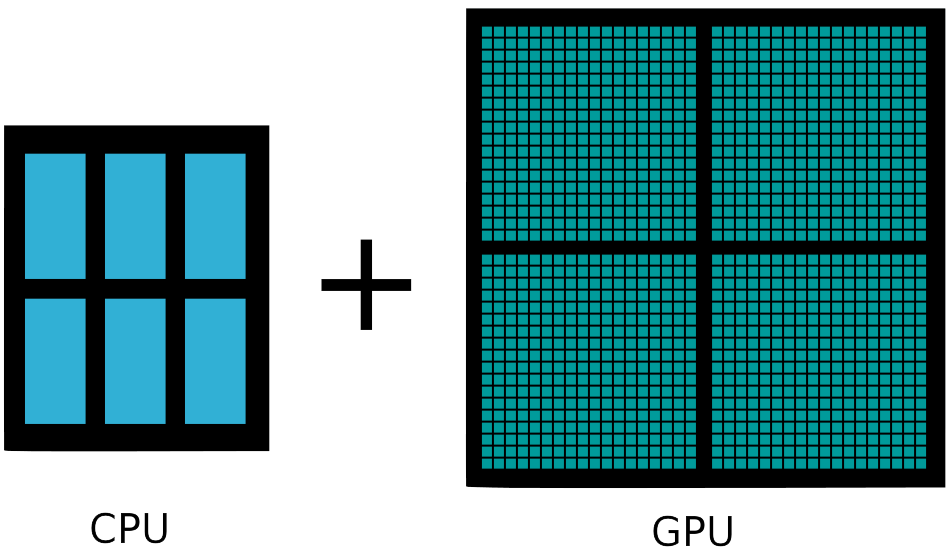
\includegraphics[width=0.9\textwidth]{Img/GPU_vs_CPU.png}
    \caption{GPU与CPU的结构对比示意图}
    \label{fig:GPU}
\end{figure}

随着GPU可编程能力、并行处理能力和应用范围方面得到不断提升和扩展,GPU已成为当前计算机系统中性能很高的部件。
因此,我们对模拟程序中的核心算法,比如PIC算法和~Symplectic算法,都进行了GPU实现。
这项工作充分利用了现有计算资源,发挥GPU的高性能计算能力,使程序在GPU与CPU之间进行协作,以提高模拟程序的运行效率。

\section{课题研究的现状}
%如何研究空间电荷效应
加速器中的束流是一个多体非线性耦合系统。
由于多体非线性耦合系统的复杂性,强流束流物理问题的研究可以从解析近似和数值模拟两个角度出发。
其中解析方法基本是在哈密顿力学的框架内加上一些必要的近似以建立起物理模型,
比如束流包络模型,单粒子运动模型等,再使用这些模型进行分析。
目前国际上流行的做法是使用非自洽的模型,比如束核模型,
对束晕产生的机制、束流集体效应等问题进行分析,给出基本的物理图像。
而数值模拟方法主要是使用束流模拟软件在计算机上进行大规模计算,对带电粒子进行跟踪和模拟。
模拟软件使用的基本模型有传输矩阵映射,PIC(Particle In Cell)等。
国际上普遍的做法是使用PIC方法求解空间电荷效应,进行粒子跟踪,得到粒子演化的图像,分析其背后的物理机制。

解析近似在某些特定的情况下可以得到较为准确的结果,可以定性的给出一些束流性质的预测和加速器设计的准则。
其优点为物理模型较为简单,计算速度快;
其缺点为对于更多的情况需要近似,与真实的加速器相差较远,对于一个具体的加速器无法给出具体定量的结论。
而数值方法依赖于具体加速器的设计,在加速器建设中起到了必不可少的作用。
其优点是可以针对具体的加速器,给出更为准确的结果;
缺点是程序编写较为繁琐,运算速度较慢。
在加速器研究中,我们一般是先用解析近似得到一个粗略的结果,再使用数值模拟进行验证和更为详细的研究。

如表\ref{tab:space_charge_code}所示,目前在国际加速器界存在着一些束流模拟软件
\cite{cern_codeList,ryne1996beam,takeda1998PARMILA,qiang1999impact,uriot2014tracewin,tanke2002dynac,shishlo2006orbit,aseev2005track}。
国内加速器界同仁大部分依然使用国外的相关软件,并且对软件内部的计算过程和算法实现并不十分了解。
但是,随着实际加速器的流强上升,我们的需求也越来越多,目前存在的软件无法完全满足我们的需求;
随着需要模拟规模越来越大,受限于已有的程序的运行效率,模拟所需要的时间也越来越长。
而且目前的软件大部分都不是开源,不方便我们根据自己的需求在底层进行改进。
国内此前对束流模拟软件的探索和开发较少,目前还没有一套成熟完备的加速器束流模拟软件。
目前,我们依托于国内近年来设计或在建C-ADS,中国散裂中子源(China Spallation Neutron Source, CSNS)等强流加速器项目,
对强流束流模拟软件进行了很多研究,
而且针对程序的效率提升方面也做出了很多探索,比如MPI,OpenMP等等CPU程序并行化,以及使用GPU并行计算。

\begin{table}
  \centering
  \caption{加速器束流模拟软件现状调研}
  \begin{tabular}{|>{\small}l|c|c|c|c|c|c|c|c|c|}
    \hline
    名称	        &开源     &界面       &并行	&后处理     &匹配	&速度 &精确度	 & 是否收费  \\
    \hline
    Parmila  	&否	   &否	   &否	&是	     &否 	&慢	 &低	     & 免费	\\
    Impact  	&是	   &否	   &是	&否	     &否	    &较快 &较高	 & 免费	\\
    TraceWin  	&否	   &是	   &是	&是	     &是	    &较快 &较高	 & 收费	\\
    Dynac  	    &是	   &否	   &否	&是	     &否	    &快     &较低	 & 免费	\\
    Orbit  	    &否	   &否	   &是	&否	     &否	    &较快 &较高	 & 免费	\\
    Track  	    &否	   &否	   &否	&否	     &否 	&较快 &较高	 & 免费	\\
    \hline
  \end{tabular}
  \label{tab:space_charge_code}
\end{table}

总之,解析近似已经不能满足现代加速器的设计和研究需求,一个可以进行精确模拟的束流模拟软件是必须的。
随着加速器束流流强的增大,模拟需要更大规模的粒子数目,而面对新的物理问题,软件所需要的功能也越来越多。
我们需要探索新的算法,编写新的粒子模拟软件,优化程序结构并提高程序运行效率,了解并掌握软件背后的计算过程。

\section{本论文主要工作}
本论文的工作主要分三个方面:
首先是根据相关的基本理论,探索强流束流动力学的物理模型和求解空间电荷效应的算法;
其次是多粒子追踪模拟软件P-TOPO(Parallelized Trace-Of-Particle-Orbit)的开发和并行优化;
最后是使用开发的束流模拟软件P-TOPO进行束流动力学研究。

本文第二章将会对强流束流动力学的基本理论进行简要介绍,其中包括束流的横向运动与纵向运动、空间电荷效应的基本理论等,并对国内外的强流加速器进行简要介绍。
第三章介绍了束流模拟程序的物理模型,以及一些相关算法和逻辑流程。其中主要介绍了包括束核模型在内的一些物理模型,以及束流模拟程序中常用的PIC算法和一种新型的Symplectic算法。
第四章介绍了模拟程序的顶层设计以及算法的实现,
包括程序总体的设计、PIC算法在GPU上和CPU集群上的实现、Symplectic保辛算法在单GPU和GPU集群上的实现,
并分别对每一种算法实现进行了正确性校验。
第五章介绍了程序中的不同算法在各个计算平台上的优化和性能测试。
第六章利用模拟程序对空间电荷效应和束流集体效应进行研究。
首先对三阶共振现象进行了一个简单模拟;
然后对加速器中束流如何自发的在共振禁带中进行演化、以及束流穿越共振禁带进行了讨论;
最后对C-ADS注入器I进行模拟研究。
第七章对论文工作进行了总结和展望。

\section{论文主要创新之处}
本文对不同的物理模型进行了比较,并开发了束流模拟软件P-TOPO。
目前在国内还没有成熟的加速器束流模拟软件,本课题的有关工作将填补国内的空白。
而且相对于其他束流模拟软件,P-TOPO在很多地方进行了创新。
比如大多数模拟软件使用飞行时间法获得加速腔的相位,而P-TOPO使用类似于实际运行中的扫相方法获得加速腔相位,虽然花费时间要更长,但是结果更加精确。
相比于其他模拟软件,我们的并行策略更为精细。我们在不同的子程序中使用了不同的并行策略,更加灵活的分配计算负载,提高了并行的效率。

除此之外,本文还在不同的空间电荷算法的并行化上进行了探索,并且在不同的并行计算架构中进行了实现。
据我们所知,Symplectic算法在GPU上的实现和PIC算法在GPU集群上的实现均为加速器界首次,这两个程序实现均取得了可观的加速比。
在PIC算法在GPU集群的实现中,我们比较了不同的并行策略下求解泊松方程的效率,并且实现并测试了新的节点间通讯方法;
而在Symplectic算法的实现中,我们针对GPU架构进行了大量优化,尤其是针对GPU的内存读写规则,重新组织了程序,使其数据吞吐速度更高。
我们还测试了Symplectic算法中每一部分的加速比和瓶颈,为下一步升级做好了准备。

最后,本文对束晕产生的机制进行了新的探索。
在对C-ADS注入器I的模拟中,验证了其设计的合理性。
本文对共振穿越的研究发现束流发射度增长几乎与束流在共振区内所停留的时间成正比,
而我们通常理解的非相干共振并不能用来解释我们研究的问题,
我们的模拟也证明了之前的理论预测,即低阶禁带被包含在高阶禁带中。
